\chapter{Random Boolean Networks}\label{rbn}
\lhead[\fancyplain{}{\bfseries\thepage}]{\fancyplain{}{\bfseries\rightmark}}


In this chapter we explain the basic concepts of Random Boolean Network proposed for the first time by Kauffman.

\section{Random Boolean Networks}
Random Boolean networks (RBNs) were introduced in
1969 by S. Kauffman as a simple model of genetic systems \cite{K1}.
Each gene was represented by a node
that has two possible states, “on” (corresponding to a
gene that is being transcribed) and “off” (corresponding
to a gene that is not being transcribed). There are altogether N nodes, and each node receives input from $K$
randomly chosen nodes, which represent the genes that
control the considered gene. Furthermore, each node is
assigned an \emph{update boolean function} that prescribes the state of
the node in the next time step, given the state of its input nodes. This update function is chosen from the set
of all possible update functions according to some probability distribution. Starting from some initial configuration, the states of all nodes of the network are updated
in parallel. Since configuration space is finite and since
dynamics is deterministic, the system must eventually return to a configuration that it has had before, and from
then on it repeats the same sequence of configurations
periodically.

\section{The model}
Let's consider a network of $N$ nodes. The state of each node at a time $t$ is given by $\sigma_i(t) \in \{0,1\}$ with $ i = 1,\dots,N$.
The $N$ nodes of the network can therefore together assume $2^N$ different states.
The number of incoming links to each node $i$ is denoted by $k_i$ and is drawn
randomly independently from the distribution $P(k_i)$.
The dynamical state of each $\sigma_i(t)$ is updated synchronously by a Boolean function $\Lambda_i$:
$$
\Lambda_i:\{0,1\}^{k_i} \to \{0,1\}
$$ 
An update function specifies
the state of a node in the next time step, given the state
of its $K$ inputs at the present time step. Since each of the
$K$ inputs of a node can be on or off, there are $M = 2^K$ possible input states.
The update function has to specify the new state of a node for each of these input states.
Consequently, there are $2^M$ different update functions.
For example let's consider a network with $K=1$, so all the functions $\Lambda_i$ receives the input from one single node. 
In general each element 
receives inputs from exactly $K$ nodes, so we have a dynamical system defined from:

\begin{equation}
\sigma_i(t+1)=\Lambda_i(\sigma_{i_1}(t),\sigma_{i_2}(t), ...,\sigma_{i_K}(t)).
\end{equation}  

So, the randomness of these network appears at two levels: in the connectivity of the network (which node is linked
to which) and the dynamics (which function is attributed to which node).

\section{Topology}
For a given number $N$ of nodes and a given number
$K$ of inputs per node, a RBN is constructed by choosing
the $K$ inputs of each node at random among all nodes.
If we construct a sufficiently large number of networks in
this way, we generate an ensemble of networks. In this
ensemble, all possible topologies occur, but their statis-
tical weights are usually different. Let us consider the
simplest possible example, $N = 2$ and $K = 1$, shown
in Figure~\ref{fig:rb}. There are 3 possible topologies.



\begin{figure}[h]
\centering
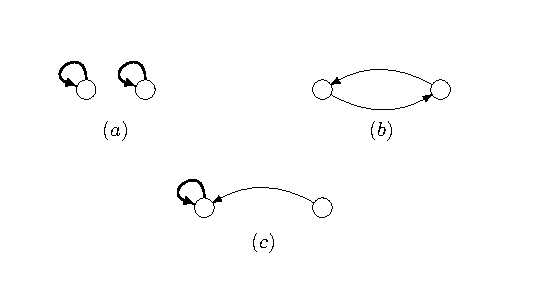
\includegraphics[scale=1.3]{figurenetworks.pdf}
\caption{Set of all possible networks with $N=2$ and $K=1$.}
\label{fig:rb}
\end{figure}

Topologies (a) and (b) have each the statistical weight $1/4$ in
the ensemble, since each of the links is connected in the
given way with probability $1/2$. Topology (c) has the
weight $1/2$, since there are two possibilities for realizing
this topology: either of the two nodes can be the one
with the self-link.


While the number of inputs of each node is fixed by
the parameter $K$, the number of outputs (i.e. of outgoing links) varies between the nodes. The mean number of
outputs must be $K$, since there must be in total the same
number of outputs as inputs. A given node becomes the
input of each of the N nodes with probability $\frac{K}{N}$ . In
the thermodynamic limit $N \to \infty$ the probability distribution of the number of outputs is therefore a Poisson
distribution:

$$
P_{out}(k) = \frac{K^k}{k!}e^{-K}
$$

\section{Dynamics}

All nodes are updated at the same time
according to the state of their inputs and to their update
function. Starting from some initial state, the network
performs a trajectory in state space and eventually arrives on an \emph{attractor}, where the same sequence of states
is periodically repeated. Since the update rule is deterministic, the same state must always be followed by the
same next state. If we represent the network states by
points in the $2^N$-dimensional state space, each of these
points has exactly one “output”, which is the successor
state. We thus obtain a graph in state space.
The size or length of an attractor is the number of
different states on the attractor. The basin of attraction
of an attractor is the set of all states that eventually
end up on this attractor, including the attractor states
themselves. The size of the basin of attraction is the
number of states belonging to it. The graph of states
in state space consists of unconnected components, each
of them being a basin of attraction and containing an
attractor, which is a loop in state space. The transient
states are those that do not lie on an attractor. They are
on trees leading to the attractors.


Let us illustrate these concepts by studying the small
$K = 1$ network shown in Figure~\ref{fig:rb2}, which consists of 4
nodes:

\begin{figure}[h]
\centering
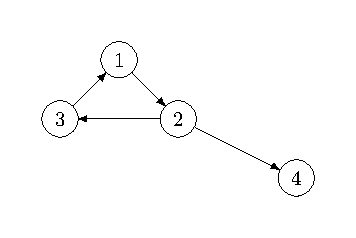
\includegraphics[scale=1.4]{figurenetworks2.pdf}
\caption{\emph{A small network with $N=4$ and $K=1$.}}
\label{fig:rb2}
\end{figure}

If we assign to the nodes 1,2,3,4 the functions invert,
invert, copy, copy, an initial state $1111$ evolves in the
following way:

$$
1111 \to 0011 \to 0100 \to 1111
$$

This is an attractor of period 3. If we interpret the bit se-
quence characterizing the state of the network as a number in binary notation, the sequence of states can also be
written as

$$
15 \to 3 \to 4 \to 15
$$

The entire state space is shown in Figure~\ref{fig:rb3}:
\begin{figure}[h]
\centering
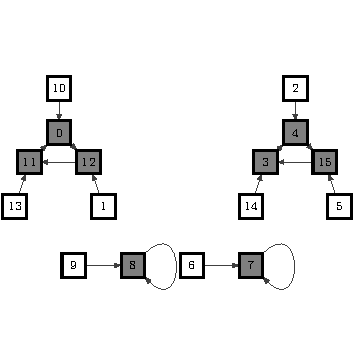
\includegraphics[scale=1.4]{fg3.pdf}
\caption{\emph{The state space of the network shown in Figure~\ref{fig:rb2}, if
the functions copy, copy, invert, invert are assigned to the four
nodes. The numbers in the squares represent states, and arrows indicate the successor of each state. States on attractors
are shaded.}}
\label{fig:rb3}
\end{figure}



There are 4 attractors, two of which are fixed points
(i.e., attractors of length $1$). The sizes of the basins of
attraction of the 4 attractors are $\Omega_1=6,\Omega_2= 6,\Omega_3 = 2,\Omega_4 = 2$. If the function
of node 1 is a constant function, fixing the value of the
node at 1, the state of this node fixes the rest of the
network, and there is only one attractor, which is a fixed
point.
\section{Phase transitions}
In RBNs, as well as in many dynamical systems, three
phases can be distinguished: \emph{ordered, chaotic, and critical}.
These phases can be identified with different methods, since
they have several unique features.
these dynamical phases is related to
“sensitivity to initial conditions”, “damage spreading”, and
“robustness to perturbations” which are different ways of
measuring the stability of a network. We can “mutate”,
“damage” or “perturb” a node of a RBN by flipping its state.
We can also change a connection between two nodes, or in
the lookup table of a node. Since nodes affect other nodes,
we can measure how much a random change affects the rest
of the network. In other words, we can measure how the
damage spreads. This can be done by comparing the evolution of a “normal” network and a “perturbed” network. In
the ordered regime, usually the damage does not spread: a
“perturbed” network “returns” to the same path of the “normal” network. This is because changes cannot propagate
from one green island to another. In the chaotic phase, these
small changes tend to propagate through the network, making it highly sensitive to perturbations \cite{K49}.
An other feature is the convergence versus divergence of the
trajectories in state space of the network dynamics. In the ordered phase, similar states tend to converge to the same state.
In the chaotic regime, similar states tend to diverge. At the
edge of chaos, nearby states tend to lie on trajectories that
neither converge nor diverge in state space.
Living systems, or computing systems, need certain stability to survive, or to keep information; but also flexibility
to explore their space of possibilities. This has lead people
to argue that life and computation occur more naturally at
the edge of chaos or at the ordered regime
close to the edge of chaos \cite{K6}\cite{K49}.
\begin{figure}[h]
\centering
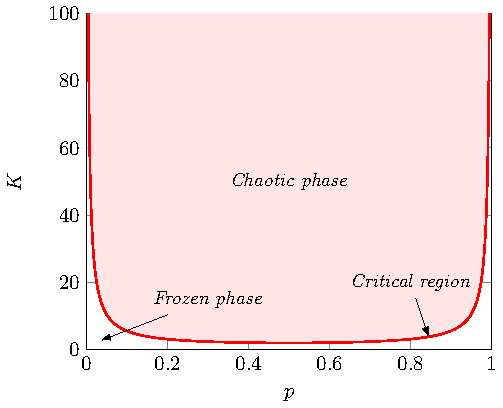
\includegraphics[scale=1.2]{images/phase-transition.pdf}
\caption{\emph{Phase diagram for the $N-K$ model. The shaded area corresponds
to the chaotic phase, whereas the white region corresponds to the chaotic phase.
The curve separating both regions is the critical phase.}}
\label{fig:ph-tr}
\end{figure}

Very early in the studies of
RBNs, people realized in simulations that the networks with
$K \le 2$ were in the ordered regime, and networks with $K \ge 3$,
were in the chaotic regime. In Figure \ref{fig:ph-tr} we can appreciate
characteristic dynamics of RBNs in different phases.
We can identify phase transitions in RBNs in different
ways. The main idea is to measure the effect of perturbations, the sensitivity to initial conditions, or damage spreading. This is analogous to Lyapunov exponents in continuous
dynamics.
The phase transitions can be statistically or analytically
obtained. Derrida and Pomeau were the first to determine
analytically that the critical phase (edge of chaos) was found
when $K = 2$ \cite{K8}\cite{K17}\cite{K21}.
following the model of Kauffman, RBN which most represent biological GRNs are those wich has $K=2$ \cite{K6}, because in the frozen phase (where $K=1$) networks are too simple to represent real regulatory networks; while in the caothic phase (where $K=3$) the time scales of the networks cycles grow exponentially, which is not biologically pheasible.
In Chapter \ref{analysis} we will see the differences in $K=1$ networks and $K=2$ networks.

\section{Perturbations}
We consider attractors in the state space as gene regulatory networks of different cells, where different attractors represent cells of different type, and where for example cancer cells lay in one specific attractor \cite{K3}\cite{K2}.
Now, if we suppose that different cell types lay in different attractors, we  suppose that the jump from an attractor to one other is given by a perturbation in the binary sequence of the genes.
So for example we take the previos network, and consider that we are in the state $12$ of the first attractor:
$$
12 \to 11 \to 0 \to 12
$$

And suddenly we change the state of the third node from $0$ to $1$:
$$
1100 \to 1110
$$

We change the system to have the state $14$ and so we jump into the second attractor:
$$
14 \to 3 \to 4 \to 15 \to 3
$$
\begin{figure}[h]
\centering
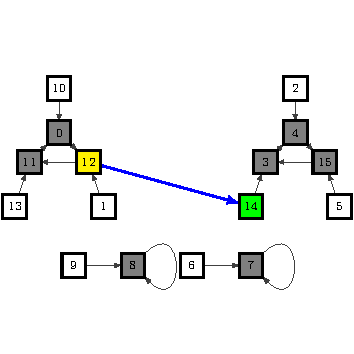
\includegraphics[scale=1.4]{fg4.pdf}
\caption{\emph{Jump from one attractor to one other in the state space.}}
\label{fig:rb4}
\end{figure}

So the branching pathways of differentiation between
attractors in a RBN in the ensembles create a directed
graph showing which attractors can be perturbed to
reach which attractors.

In fact, if we consider all the possible stochastic perturbations in the binary sequence of the genes, we can get the all the possible transitions between the attractors, and what we obtain is an other network, where the nodes are the attractors and the frequencies of transitions can be used to build a random walk on this network\cite{K2}.


